\section{Middleware and Telemetry Validation}
\label{sec:middleware_telemetry_validation}

\subsection{Telemetry Test Conditions}

Four representative operating conditions were selected: mission operation without vision processing, a static no-vision baseline, Edge processing and Ground processing. Invalid, contaminated and incomplete attempts were excluded using the Phase C selection record. One complete run represented each condition, so the comparison was descriptive rather than statistical.

\subsection{Telemetry Continuity Results}

Table~\ref{tab:middleware_telemetry_summary} summarises the message activity in the selected runs. Telemetry remained active in every condition. The Ground run produced the lowest mean message rate, 1.53~Hz, and the largest observed message gap, 3788.4~ms. The Edge result, 2.06~Hz, remained closer to the two no-vision conditions.

\begin{table}[htbp]
    \centering
    \caption{Telemetry continuity for the four selected operating conditions.}
    \label{tab:middleware_telemetry_summary}
    \begin{tabular}{lrrr}
        \toprule
        Condition & Messages & Mean rate (Hz) & Maximum gap (ms) \\
        \midrule
        C0 mission/no vision & 274 & 2.28 & 2243.2 \\
        C1 static/no vision & 253 & 2.11 & 1994.1 \\
        C2 Edge & 247 & 2.06 & 2354.9 \\
        C3 Ground & 184 & 1.53 & 3788.4 \\
        \bottomrule
    \end{tabular}
\end{table}

% This descriptive figure can be removed if the final report needs a table-only layout.
\begin{figure}[htbp]
    \centering
    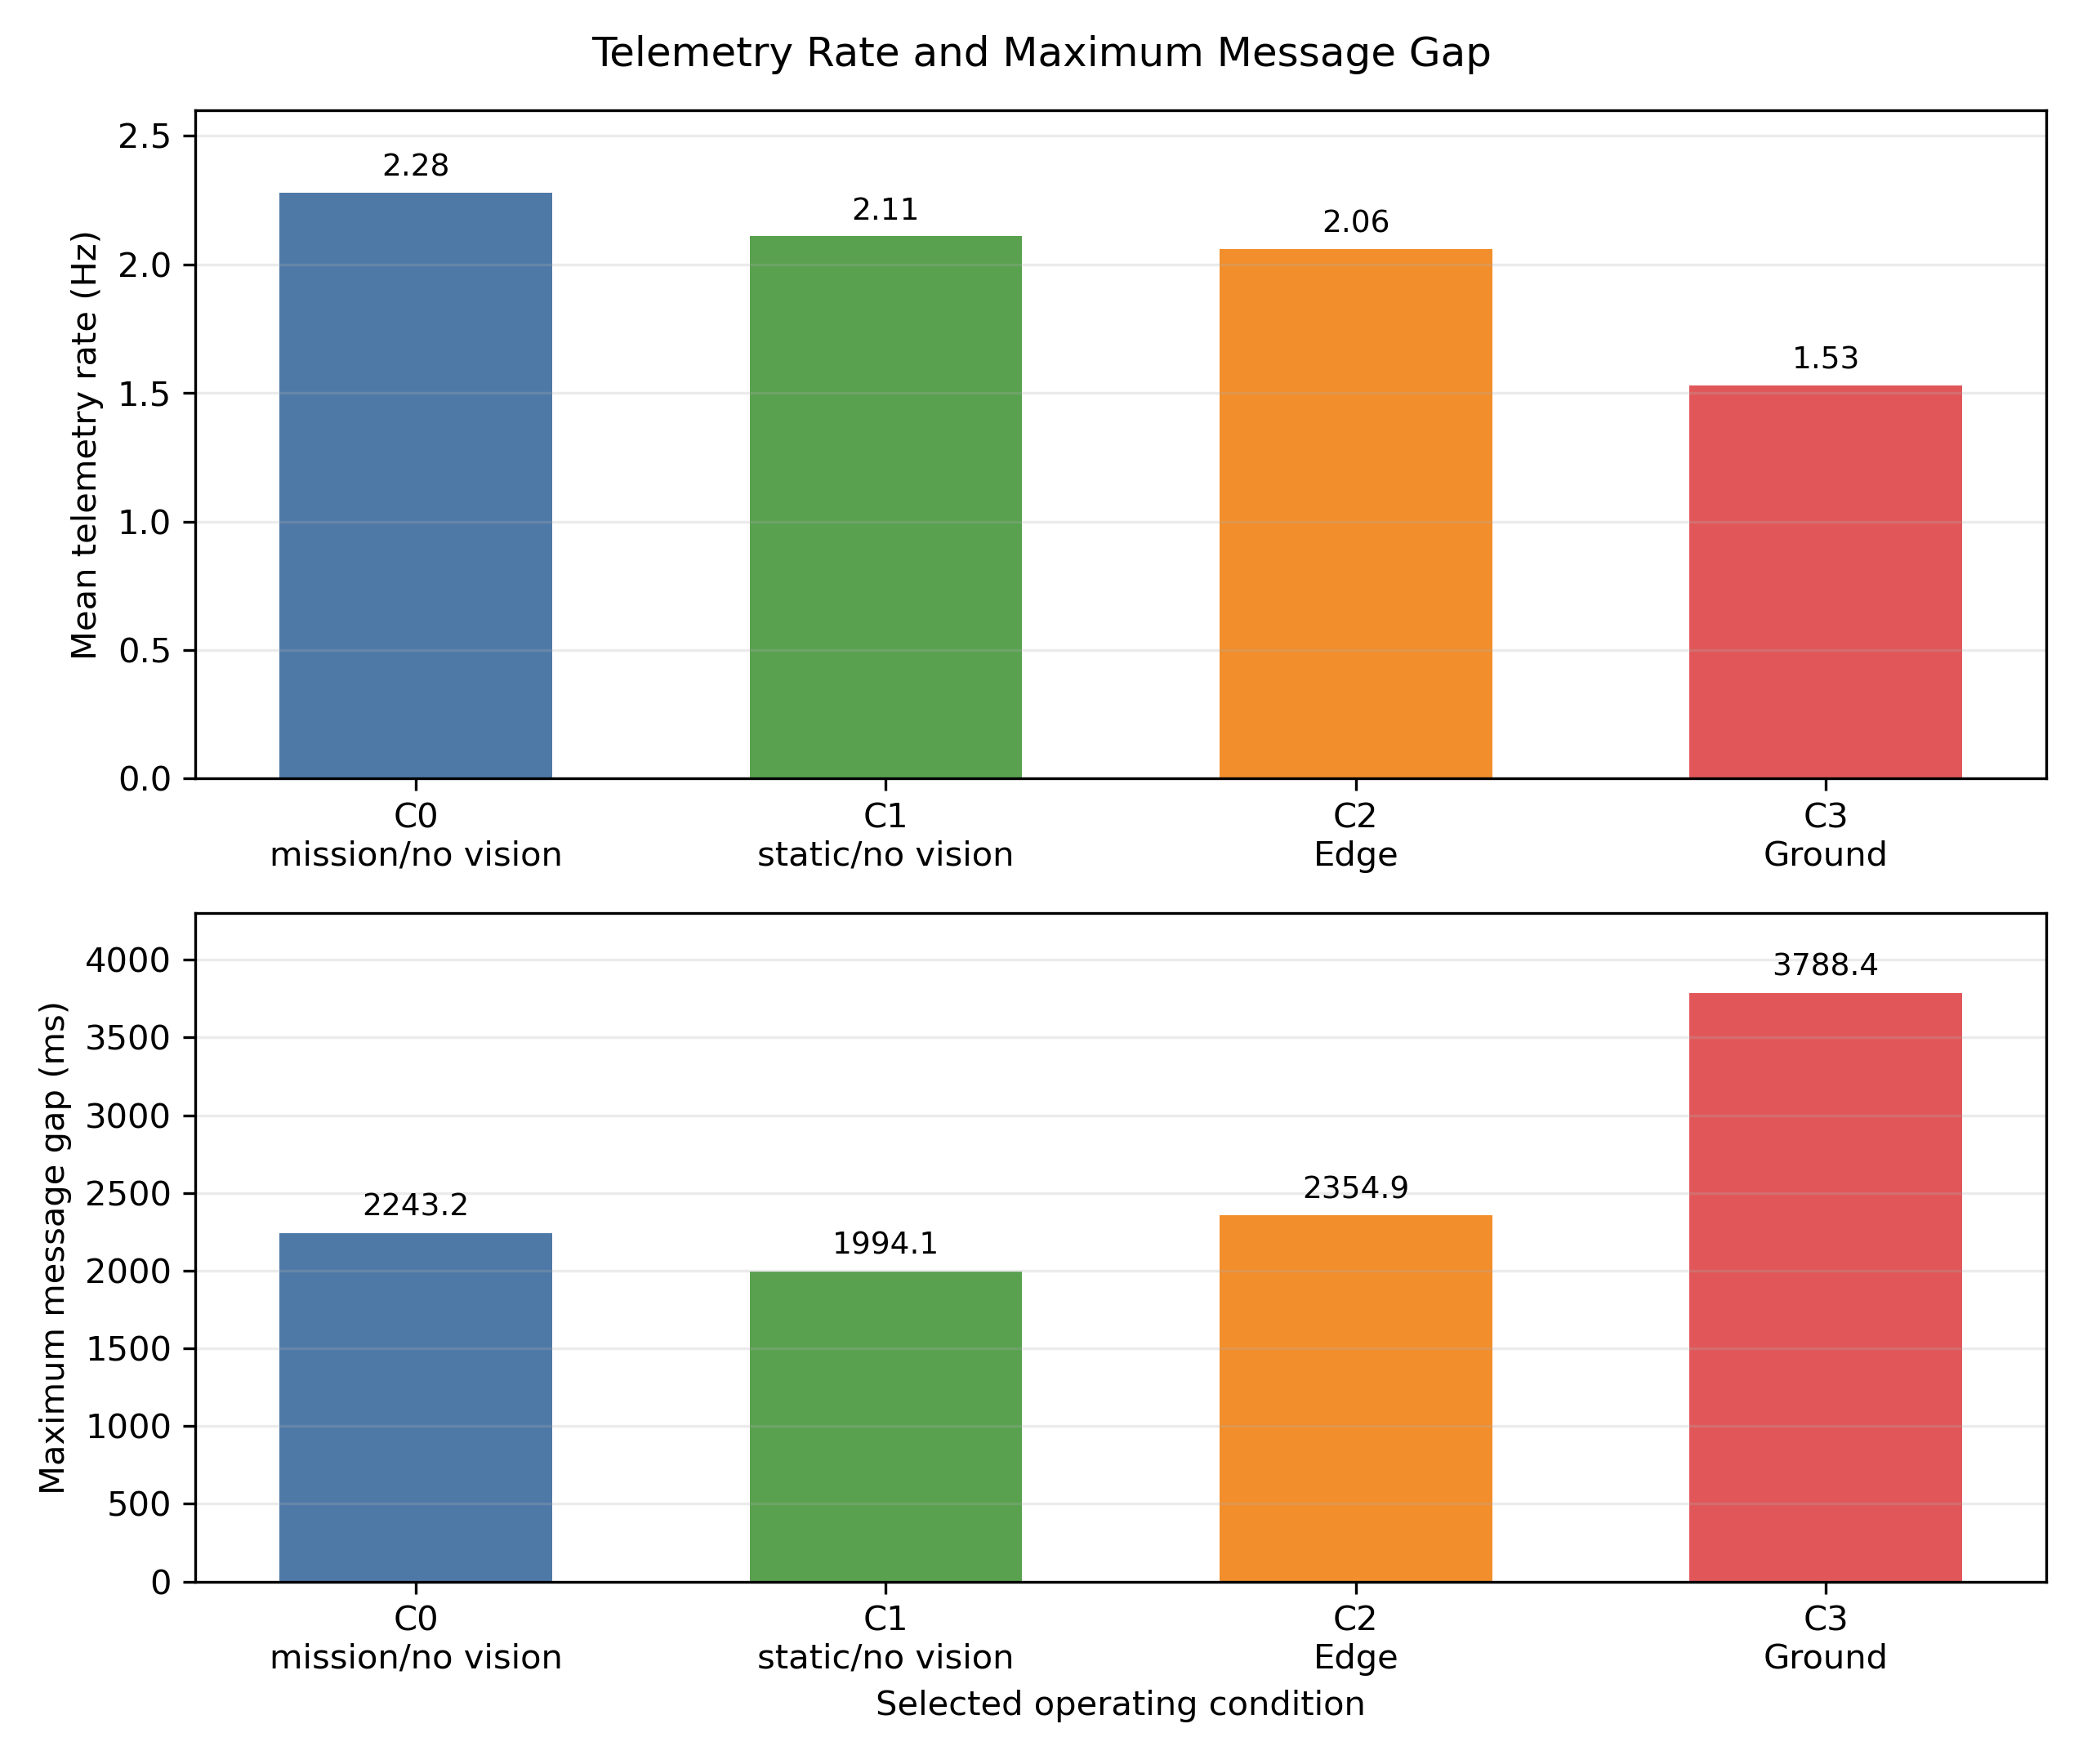
\includegraphics[width=0.82\textwidth]{images/chapter5/middleware/telemetry_rate_and_gap.png}
    \caption{Mean telemetry rate and maximum message gap in the selected Phase C runs.}
    \label{fig:middleware_telemetry_rate_gap}
\end{figure}

This pattern is consistent with additional traffic or processing contention during Ground operation. However, the experiment did not isolate image transfer as the sole cause, and only one selected run represented each condition.

\subsection{Middleware Validation Summary}

Middleware communication remained operational across the four selected conditions, although the Ground run showed the greatest reduction in telemetry continuity. This result provides useful context for the later Edge and Ground application comparison. Broader experiments with repeated runs would still be needed before making statistical or general causal claims.
